\documentclass{ximera}

\graphicspath{  
{./}
{./whoAreYou/}
{./drawingWithTheTurtle/}
{./bisectionMethod/}
{./circles/}
{./anglesAndRightTriangles/}
{./lawOfSines/}
{./lawOfCosines/}
{./plotter/}
{./staircases/}
{./pitch/}
{./qualityControl/}
{./symmetry/}
{./nGonBlock/}
}


%% page layout
\usepackage[cm,headings]{fullpage}
\raggedright
\setlength\headheight{13.6pt}


%% fonts
\usepackage{euler}

\usepackage{FiraMono}
\renewcommand\familydefault{\ttdefault} 
\usepackage[defaultmathsizes]{mathastext}
\usepackage[htt]{hyphenat}

\usepackage[T1]{fontenc}
\usepackage[scaled=1]{FiraSans}

%\usepackage{wedn}
\usepackage{pbsi} %% Answer font


\usepackage{cancel} %% strike through in pitch/pitch.tex


%% \usepackage{ulem} %% 
%% \renewcommand{\ULthickness}{2pt}% changes underline thickness

\tikzset{>=stealth}

\usepackage{adjustbox}

\setcounter{titlenumber}{-1}

%% journal style
\makeatletter
\newcommand\journalstyle{%
  \def\activitystyle{activity-chapter}
  \def\maketitle{%
    \addtocounter{titlenumber}{1}%
                {\flushleft\small\sffamily\bfseries\@pretitle\par\vspace{-1.5em}}%
                {\flushleft\LARGE\sffamily\bfseries\thetitlenumber\hspace{1em}\@title \par }%
                {\vskip .6em\noindent\textit\theabstract\setcounter{question}{0}\setcounter{sectiontitlenumber}{0}}%
                    \par\vspace{2em}
                    \phantomsection\addcontentsline{toc}{section}{\thetitlenumber\hspace{1em}\textbf{\@title}}%
                     }}
\makeatother



%% thm like environments
\let\question\relax
\let\endquestion\relax

\newtheoremstyle{QuestionStyle}{\topsep}{\topsep}%%% space between body and thm
		{}                      %%% Thm body font
		{}                              %%% Indent amount (empty = no indent)
		{\bfseries}            %%% Thm head font
		{)}                              %%% Punctuation after thm head
		{ }                           %%% Space after thm head
		{\thmnumber{#2}\thmnote{ \bfseries(#3)}}%%% Thm head spec
\theoremstyle{QuestionStyle}
\newtheorem{question}{}



\let\freeResponse\relax
\let\endfreeResponse\relax

%% \newtheoremstyle{ResponseStyle}{\topsep}{\topsep}%%% space between body and thm
%% 		{\wedn\bfseries}                      %%% Thm body font
%% 		{}                              %%% Indent amount (empty = no indent)
%% 		{\wedn\bfseries}            %%% Thm head font
%% 		{}                              %%% Punctuation after thm head
%% 		{3ex}                           %%% Space after thm head
%% 		{\underline{\underline{\thmname{#1}}}}%%% Thm head spec
%% \theoremstyle{ResponseStyle}

\usepackage[tikz]{mdframed}
\mdfdefinestyle{ResponseStyle}{leftmargin=1cm,linecolor=black,roundcorner=5pt,
, font=\bsifamily,}%font=\wedn\bfseries\upshape,}


\ifhandout
\NewEnviron{freeResponse}{}
\else
%\newtheorem{freeResponse}{Response:}
\newenvironment{freeResponse}{\begin{mdframed}[style=ResponseStyle]}{\end{mdframed}}
\fi



%% attempting to automate outcomes.

%% \newwrite\outcomefile
%%   \immediate\openout\outcomefile=\jobname.oc
%% \renewcommand{\outcome}[1]{\edef\theoutcomes{\theoutcomes #1~}%
%% \immediate\write\outcomefile{\unexpanded{\outcome}{#1}}}

%% \newcommand{\outcomelist}{\begin{itemize}\theoutcomes\end{itemize}}

%% \NewEnviron{listOutcomes}{\small\sffamily
%% After answering the following questions, students should be able to:
%% \begin{itemize}
%% \BODY
%% \end{itemize}
%% }
\usepackage[tikz]{mdframed}
\mdfdefinestyle{OutcomeStyle}{leftmargin=2cm,rightmargin=2cm,linecolor=black,roundcorner=5pt,
, font=\small\sffamily,}%font=\wedn\bfseries\upshape,}
\newenvironment{listOutcomes}{\begin{mdframed}[style=OutcomeStyle]After answering the following questions, students should be able to:\begin{itemize}}{\end{itemize}\end{mdframed}}



%% my commands

\newcommand{\snap}{{\bfseries\itshape\textsf{Snap!}}}
\newcommand{\flavor}{\link[\snap]{https://snap.berkeley.edu/}}
\newcommand{\mooculus}{\textsf{\textbf{MOOC}\textnormal{\textsf{ULUS}}}}


\usepackage{tkz-euclide}
\tikzstyle geometryDiagrams=[rounded corners=.5pt,ultra thick,color=black]
\colorlet{penColor}{black} % Color of a curve in a plot



\ifhandout\newcommand{\mynewpage}{\newpage}\else\newcommand{\mynewpage}{}\fi



\title{Design in a line}

\author{Bart Snapp}



\begin{document}
\begin{abstract}
  We introduce freize patterns.
\end{abstract}
\maketitle

In design and architecture, a \index{frieze pattern}\textit{frieze},
pronounced ``freeze,'' is a horizontal band that is found near the
ceiling or roof. It is often decorated with a repeating design. Let's
see some examples:
\begin{center}
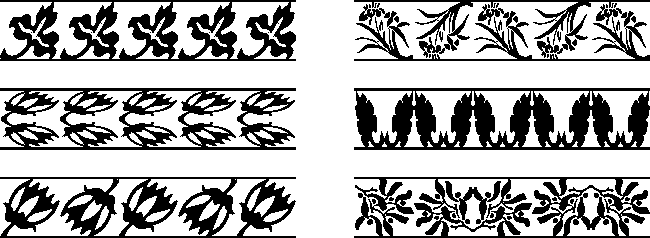
\includegraphics{fpfrieze.pdf}
\end{center}
In each case, the pattern above can be thought of as an infinite strip
with the pattern continuing indefinitely.  Frieze patterns often have
symmetry in their structure. While in real-life, the symmetry would
not be perfect, it is useful in mathematics to simplify reality by
replacing the real patterns by idealized designs.  In this chapter, we
will study the symmetry of frieze patterns. At this point we will
refrain from giving a rigorous definition of a \textit{frieze
  pattern}. Instead, this will be a result of our work in this
chapter.

\section{Symmetries}

\subsection*{Translations}\index{translation}

Perhaps the most apparent symmetry that frieze patters can exhibit is
symmetry through \textit{horizontal translations}:
\begin{center}

\includegraphics{fptrans.pdf}
\end{center}
We will not only insist that a frieze pattern always have
translational symmetry, but we will also insist that such a
translation is \textit{discrete}, meaning that it occurs in distinct
``hops'' of some minimal distance. So, for example, the while the
following patterns have minimal discrete translations, 
\begin{center}

\includegraphics{fptransDis.pdf}
\end{center}
this pattern
\begin{center}

\includegraphics{fptransNot.pdf}
\end{center}
does not, and hence will not technically be considered a frieze
pattern. To be completely explicit: 
\begin{center}
\textbf{All frieze patterns have symmetry through a minimal discrete
  horizontal translation.}
\end{center}
\begin{definition}\index{minimal cell}
A \textbf{minimal cell} is the smallest slice of a frieze
pattern that will produce the entire frieze pattern through horizontal
translations.
\end{definition}

\begin{warning}
The minimal cell of a frieze pattern is not unique! Consider
\begin{center}
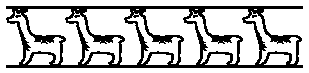
\includegraphics{fptransMinEG.pdf}
\end{center}
both
\begin{center}

\includegraphics{fptransMinEGCell.pdf} \qquad\text{and}\qquad  
\includegraphics{fptransMinEGCell2.pdf}
\end{center}
are minimal cells.
\end{warning} 



\subsection*{Horizontal Reflections}\index{horizontal reflection}

Frieze patterns can have symmetry through \textit{horizontal reflections}:
\[

\includegraphics{fphoriz.pdf}
\]
Some frieze patterns have symmetry through horizontal reflections, while
others don't.
\begin{question} 
Can you identify the frieze patterns below with symmetry through
horizontal reflections?
\[
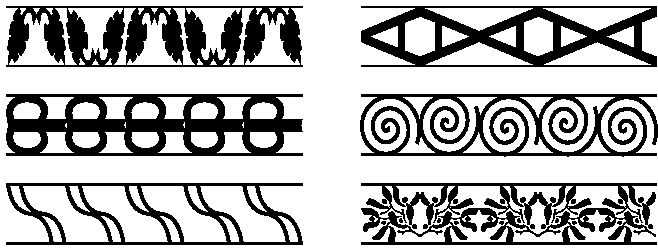
\includegraphics{fpfriezeHoriz.pdf}
\]
\end{question}

\begin{warning}
Remember: A horizontal reflection reflects across a vertical line!
\end{warning}



\subsection*{Vertical Reflections}\index{vertical reflection}


Frieze patterns can have symmetry through \textit{vertical reflections}:
\[

\includegraphics{fpvertical.pdf}
\]

\begin{question}
Can you identify the frieze patterns below with symmetry through
vertical reflections?
\[
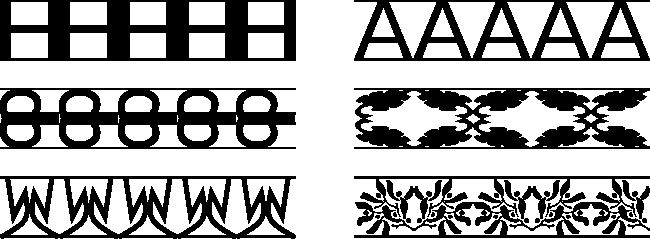
\includegraphics{fpfriezeVert-Horiz.pdf}
\]
\end{question}

\begin{warning}
Remember: A vertical reflection reflects across a horizontal
line!
\end{warning}




\subsection*{Glide Reflections}\index{glide reflection}

Frieze patterns can have symmetry through \textit{glide reflections}:
\[

\includegraphics{fpglide.pdf}
\]

\begin{question}
Can you identify the frieze patterns below with symmetry through glide
reflections?
\[
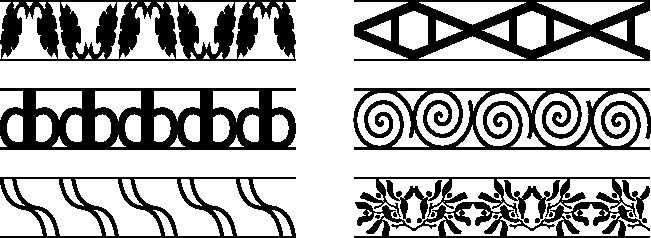
\includegraphics{fpfriezeGlide.pdf}
\]
\end{question}

\begin{question}
If a frieze pattern has symmetry through translations and vertical
reflections, must it have symmetry through glide reflections?
\end{question}





\subsection*{Rotations}\index{rotations}

Finally, frieze patterns can have symmetry through $180^\circ$
rotations.
\[
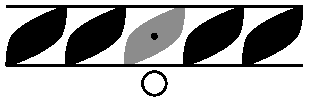
\includegraphics{fprot.pdf}
\]

\begin{question}
Can you identify the frieze patterns below that have symmetry through
$180^\circ$ rotations?
\[
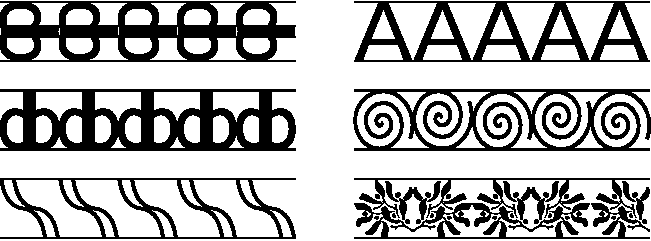
\includegraphics{fpfriezeRot.pdf}
\]
\end{question}

\begin{question}
Suppose you have a frieze pattern with symmetry through both glide
reflections and $180^\circ$ rotations. Must this pattern also have
symmetry through horizontal reflections?
\end{question}



\begin{question}
Imagine that you have a frieze pattern that has symmetry through
horizontal reflections and $180^\circ$ rotations, but not through
vertical reflections. Could the center of the rotation be on the
vertical line that defines the reflection?
\end{question}

I think I'll step in and give you a big hint. Consider the following
set of pictures and mysterious symbols:
\[
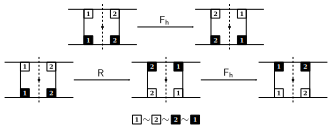
\includegraphics{friezeRotRefCent.pdf}
\]
\begin{question}
Can you explain what these pictures are trying to express?
\end{question}



%% \newpage

%% \problems
%% \begin{enumerate}
%% \item Explain what it means for a frieze pattern to have symmetry
%%   through horizontal translations. Feel free to draw pictures to help out.
%% \item Explain what it means for a frieze pattern to have symmetry
%%   through horizontal reflections. Feel free to draw pictures to help out.
%% \item Explain what it means for a frieze pattern to have symmetry
%%   through vertical reflections. Feel free to draw pictures to help out.
%% \item Explain what it means for a frieze pattern to have symmetry
%%   through glide reflections. Feel free to draw pictures to help out.
%% \item Explain what it means for a frieze pattern to have symmetry
%%   through $180^\circ$ rotations. Feel free to draw pictures to help out.
%% \item Draw a frieze pattern that exhibits symmetry through horizontal
%%   translations and identify $3$ different minimal cells.
%% \item Draw a frieze pattern that exhibits symmetry through horizontal
%%   translations and glide reflections, but does not have symmetry
%%   through any other transformation. Be sure to identify a minimal
%%   cell.
%% \item Draw a frieze pattern that exhibits symmetry through horizontal
%%   translations and horizontal reflections, but does not have symmetry
%%   through any other transformation. Be sure to identify a minimal
%%   cell.
%% \item Draw a frieze pattern that exhibits symmetry through horizontal
%%   translations and $180^\circ$ rotations, but does not have symmetry
%%   through any other transformation. Be sure to identify a minimal
%%   cell.
%% \item Draw a frieze pattern that exhibits symmetry through horizontal
%%   translations, vertical reflections, and glide reflections, but does
%%   not have symmetry through any other transformation. Be sure to
%%   identify a minimal cell.
%% \item Draw a frieze pattern that exhibits symmetry through horizontal
%%   translations, horizontal reflections, glide reflections, and
%%   $180^\circ$ rotations, but does not have symmetry through any other
%%   transformation. Be sure to identify a minimal cell.
%% \item Draw a frieze pattern that exhibits symmetry through horizontal
%%   translations, horizontal reflections, vertical reflections, glide
%%   reflections, and $180^\circ$ rotations. Be sure to identify a
%%   minimal cell.
%% \item Consider the following frieze pattern:
%% \[
%% 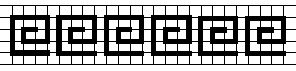
\includegraphics{fpGraphEx1.pdf}
%% \]
%% Explicitly write down the matrices for the symmetries of this
%% pattern. Explain your reasoning.
%% \item Consider the following frieze pattern:
%% \[
%% 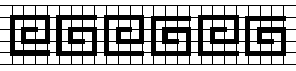
\includegraphics{fpGraphEx2.pdf}
%% \]
%% Explicitly write down the matrices for the symmetries of this
%% pattern. Explain your reasoning.
%% \item Consider the following frieze pattern:
%% \[
%% 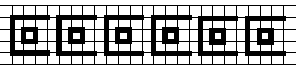
\includegraphics{fpGraphEx3.pdf}
%% \]
%% Explicitly write down the matrices for the symmetries of this
%% pattern. Explain your reasoning.
%% \item Consider the following frieze pattern:
%% \[
%% 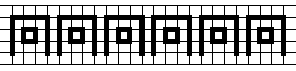
\includegraphics{fpGraphEx4.pdf}
%% \]
%% Explicitly write down the matrices for the symmetries of this
%% pattern. Explain your reasoning.
%% \item Consider the following frieze pattern:
%% \[
%% 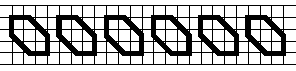
\includegraphics{fpGraphEx5.pdf}
%% \]
%% Explicitly write down the matrices for the symmetries of this
%% pattern. Explain your reasoning.
%% \item Consider the following frieze pattern:
%% \[
%% 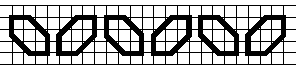
\includegraphics{fpGraphEx6.pdf}
%% \]
%% Explicitly write down the matrices for the symmetries of this
%% pattern. Explain your reasoning.
%% \item Consider the following frieze pattern:
%% \[
%% 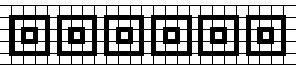
\includegraphics{fpGraphEx7.pdf}
%% \]
%% Explicitly write down the matrices for the symmetries of this
%% pattern. Explain your reasoning.
%% \item Can you exhibit a frieze pattern with 
%% symmetry through $180^\circ$ rotations but not through glide reflections?
%% If so, present such a pattern and identify a minimal translation
%% cell. If not, explain why not.
%% \item Can you exhibit a frieze pattern with 
%% symmetry through horizontal reflections but not through glide reflections?
%% If so, present such a pattern and identify a minimal translation
%% cell. If not, explain why not.
%% \item Can you exhibit a frieze pattern with 
%% symmetry through vertical reflections but not through glide reflections?
%% If so, present such a pattern and identify a minimal translation
%% cell. If not, explain why not.
%% \item Can you exhibit a frieze pattern with 
%% symmetry through horizontal reflections and $180^\circ$ rotations but not through glide reflections?
%% If so, present such a pattern and identify a minimal translation
%% cell. If not, explain why not.

\end{document}
